\chapter{Background}

\section{Classical Planning}

Classical Planning is achieving a significant advance in the recent years due to the success of heuristic search.
The input problem to a Classical Planning solver (a \emph{planner}) is a 5-tuple 
$\Pi=\brackets{P,O,I,G,A}$ where $P$ defines a set of first-order predicates, $O$ is a set of symbols called \emph{objects}, $I$ is the initial state, $G$ is a set of goal conditions, and $A$ is a set of actions which defines the state transitions in the search space.
A state is an assignment of boolean values to the set of propositional variables, while a condition is a partial assignment that assigns values only to a subset of propositions.
Each proposition is an instantiation of a predicate with objects.
% 
% 
Lifted action schema $a \in A$ is a 5-tuple
$\brackets{\mbox{\textit{params}}, \mbox{\textit{pre}}, e^+, e^-, c}$
where each element means the set of parameters, preconditions,
add-effects, delete-effects and the cost, respectively.
% Precondition defines a situation when the action is applicable. Add/delete-effects define how the action modifies the state by adding/deleting propositions.
% In most cases, an action and its elements are \emph{lifted} (parameterized) by \textit{params}.
Parameter substitution using objects in $O$ instantiates \emph{ground actions}.
When $c$ is not specified, it is usually assumed $c=1$.
These inputs are described in a PDDL modeling language \cite{McDermott00} and its extensions.

\refig{8puzzle-pddl} shows one possible representation of a state in
3x3 sliding tile puzzle (8-puzzle) in the First Order Logic formula, and the
representation of the same state using PDDL.

\begin{figure}[htb]
\centering
\begin{minipage}[c]{0.2\linewidth}
 \begin{align*}
        & Empty(x_0, y_0)          \\
  \land & At   (x_1, y_0, panel_6) \\
  \land & Up   (y_0, y_1)          \\
  \land & Down (y_1, y_0)          \\
  \land & Right(x_0, x_1)          \\
  \land & Left (x_1, x_0)       \ldots 
 \end{align*}
\end{minipage}
\begin{minipage}[c]{0.4\linewidth}
 \begin{lstlisting}
  (empty x0 y0)
  (at    x1 y0 panel6)
  (up    y0 y1)
  (down  y1 y0)
  (right x0 x1)
  (left  x1 x0)...
 \end{lstlisting}
\end{minipage}
\begin{minipage}[c]{0.3\linewidth}
 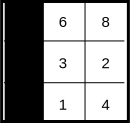
\includegraphics[width=\linewidth]{img/pddl/8puzzle-standard.pdf}
\end{minipage}
\caption{One possible state representation of a
3x3 sliding tile puzzle (8-puzzle) in the first order logic formula and its
corresponding PDDL notation. It contains predicate symbols 
\pddl{empty}, \pddl{up}, \pddl{down}, \pddl{left}, \pddl{right}, \pddl{at} as well as
object symbols such as \pddl{x}$_i$, \pddl{y}$_i$, \pddl{panel}$_j$ for $i \in \braces{0..3}$ and $j\in \braces{1..8}$.
}
\label{8puzzle-pddl}
\end{figure}

\begin{figure}[htb]
\begin{minipage}[c]{0.3\linewidth}
 \small
\begin{align*}
 \text{When}  & \quad Empty(x, y_{old}) \\
        & \land at(x, y_{new}, p) \\
        & \land up(y_{new}, y_{old}) ; \\
 \text{then}  & \quad \lnot Empty(x,y_{old}) \\
        & \land Empty(x,y_{new}) \\
        & \land \lnot at(x, y_{new}, p) \\
        & \land at(x, y_{old}, p)
\end{align*}
\end{minipage}
\begin{minipage}[c]{0.42\linewidth}
 \begin{lstlisting}
(:action slide-up ...
 :precondition
 (and (empty ?x ?y-old)
      (at ?x ?y-new ?p)
      (up ?y-new ?y-old))
 :effects
 (and (not (empty ?x ?y-old))
      (empty ?x ?y-new)
      (not (at ?x ?y-new ?p))
      (at ?x ?y-old ?p)))
 \end{lstlisting}
\end{minipage}
\begin{minipage}[c]{0.25\linewidth}
 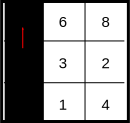
\includegraphics[width=\linewidth]{img/pddl/8puzzle-standard-tile7.pdf}
\end{minipage}
\caption{One possible action representation of sliding up a tile in 3x3
sliding tile puzzle in (left) the first order logic formula and (middle)
its corresponding PDDL notation. In addition to
\refig{8puzzle-pddl}, it further contains an action symbol
\pddl{slide-up}.  } \label{8puzzle-action-pddl}
\end{figure}


The task of a planning problem is to find a path from the initial state
$I$ to some goal state $s^*\supseteq G$, using the state transition
rules in $A$. A state $s$ can be transformed into a new state $t$ by
applying a ground action $a$ when $s\supseteq \mbox{\textit{pre}}$, and
then $t=(s\setminus e^-)\cup e^+$ \cite{McDermott00}. This transition
can also be viewed as applying a state transition function $a$ to $s$,
which can be written as $t=a(s)$.

% Finally, a \emph{plan}  $P$ is a sequence of ground actions
% $\brackets{a_0,a_1\ldots a_n}$, which, when applied to $I$, results in a
% goal state $s^*\supseteq G$.\todo*{seems that defining ``path'' was unnecessary(?)}
% Finally, a path is a sequence of ground actions $\brackets{a_0,a_1\ldots
% a_n}$. When a path leads to some goal $s^*$ from $I$, it is called a
% \emph{plan} of $\Pi$.

\sota planners solve this problem as a path finding problem on a
implicit graph defined by the state transition rules. They usually
employ forward state space heuristic search, such as \astar (for finding
the shortest path) or Greedy Best-First Search (for finding a suboptimal
path more quickly). Thanks to the variety of successful
domain-independent heuristic functions
\cite{Helmert2009,sievers2012efficient,helmert2007flexible,bonet2013admissible,hoffmann01,Helmert04,richter2008landmarks},
current \lsota planners can scale to larger problems which requires to
find a plan consisting of more than 1000 steps \cite{Asai2015}.

% To name a few heuristics, they are (admissible) LM-cut heuristics \cite{Helmert2009}, Pattern Database (PDB) heuristics \cite{sievers2012efficient}, Merge-and-shrink heuristics \cite{helmert2007flexible} or LP-relaxation heuristics \cite{bonet2013admissible}, or (inadmissible) FF heuristics \cite{hoffmann01}, Causal Graph heuristic \cite{Helmert04} and Landmark-Count heuristics \cite{richter2008landmarks}.

